\documentclass[10pt,a4paper]{article}
\usepackage[utf8]{inputenc}
\usepackage[ngerman]{babel}
\usepackage{amsmath}
\usepackage{amsfonts}
\usepackage{amssymb}
\usepackage{mathtools}
\usepackage{microtype}
\usepackage{authblk}
\usepackage{titlesec}

% section title formating
\renewcommand{\thesection}{\Roman{section}}
\titleformat{\section}[block]{\normalsize\bfseries}{\thesection.}{1em}{\MakeUppercase}
\titlespacing*{\section}{0pt}{11pt plus 2pt minus 2pt}{11pt plus 2pt minus 2pt}

\renewcommand{\thesubsection}{\arabic{section}.\Alph{subsection}}
\titleformat{\subsection}{\normalsize\bfseries}{\thesubsection}{1em}{}
\titlespacing*{\subsection}{0pt}{11pt plus 2pt minus 2pt}{11pt plus 2pt minus 2pt}

\renewcommand{\thesubsubsection}{\thesubsection.\arabic{subsubsection}}
\titleformat{\subsubsection}{\normalsize\itshape}{\thesubsubsection}{1em}{}
\titlespacing*{\subsubsection}{0pt}{11pt plus 2pt minus 2pt}{11pt plus 2pt minus 2pt}
   
% custom macros
\newcommand{\mydef}[1]{\textls{#1}}
\newcommand{\nul}{\textrm{---}}
\newcommand{\trans}{^\mathsf{T}}

% %%%%%%%
% title %
% %%%%%%%

\title{Verwendung von Ephemeridenparametern im Kontext von GNSS}
\author{Hendrik Meier}

\affil{Oberuhldingen}
\renewcommand\Affilfont{\itshape}

\date{November 2025}


% %%%%%%%%%%
% document %
% %%%%%%%%%%

\begin{document}
\maketitle

Dieser Aufsatz stellt die mathematischen Mittel bereit, um mit Hilfe der von einem GNSS-Satelliten übermittelten auf Keplerbahn\-parametrisierung basierenden Ephemeridendaten die Position der GNSS-Antenne zu berechnen.
Die genannte Form der Parametrisierung betrifft insbesondere die Systeme GPS, Galileo, QZSS und Beidou.


\section{Elliptische Bahnen im Keplerproblem}

\subsection{Bewegung im Zentralpotential}

Die Bewegung eines Satelliten mit Einheitsmasse um einen sehr viel schwereren Zentralkörper ist durch die Lagrange-Funktion
\begin{align}
	\mathcal{L}(q, \dot{q}) &=
	\frac{1}{2} |\dot{q}|^2 - V(|q|)
\end{align}
gegeben.
Darin stellen die Koordinaten $q\in\mathbb{R}^3$ und $\dot{q}\in\mathrm{T}_q\mathbb{R}^3\cong\mathbb{R}^3$ Position und Geschwindigkeit des Satelliten dar.

Die Drehimpuls\-erhaltung impliziert, dass die Satellitenbewegung in der Ebene stattfindet, die durch die jeweils gegenwärtigen Werte von $q$ und $\dot{q}$ bestimmt ist.
(Wir nehmen im Folgenden durchweg an, dass der Drehimpuls $q\times\dot{q}\neq 0$ ist.)
In dieser Ebene führen wir Polarkoordinaten
\begin{align}
	\label{eq:polar_coord}
	x &= r \cos\Phi\ ,\quad y = r \sin\Phi
\end{align}
ein, in denen die Lagrange-Funktion die Form
\begin{align}
	\mathcal{L}(r, \Phi; \dot{r}, \dot{\Phi}) &=
	\frac{1}{2} \dot{r}^2 + 
	\frac{1}{2} r^2\dot{\Phi}^2 - V(r)
\end{align}
annimmt.
Für die radiale Lagrange-Gleichung folgt
\begin{align}
	\ddot{r} &=	 
	\frac{L^2}{r^3} - \partial_rV(r)	
\end{align}
mit dem erhaltenen Drehimpuls~$L=r^2\dot{\Phi}$, dem kanonischen Impuls zur zyklischen Variablen~$\Phi$.
Multiplikation der radialen Bewegungsgleichung mit $\dot{r}$ liefert die Energieerhaltung,
\begin{align}
	\frac{d}{dt}\left[
		\frac{1}{2} \dot{r}^2
		+ \frac{L^2}{2r^2} + V(r)
	\right] &= 0
	\ ,
\end{align}
und wir erhalten
\begin{align}
	\dot{r}& = \sqrt{2 E - \frac{L^2}{r^2} - 2 V(r)}
\end{align}
und nach Substitution $\dot{r}=(d\Phi/dt)(d\Phi/dr)^{-1}=(L/r^2)(d\Phi/dr)^{-1}$ schließlich
\begin{align}
	\label{eq:dphidr}
	\frac{d\Phi}{dr} &= \frac{L/r}{\sqrt{2 E r^{2} - L^2 - 2 V(r) r^{2}}}
	\ .
\end{align}

\subsection{Lösung des Keplerproblems}
\label{ssec:kepler_solution}

Für das Gravitationspotential
\footnote{Es ist $\mu = G M_\oplus$ mit der Erdmasse~$M_\oplus$ und der Gravitationskonstanten $G$. Der WGS84-Wert ist $\mu_{\mathrm{WGS}84} = 3,986004418\cdot 10^{14} \mathrm{m^3/s^2}$.}
\begin{align}
	V(r) &= -\frac{\mu}{r}
\end{align}
mit der spezifischen Graviation~$\mu$ integrieren wir Gl.~(\ref{eq:dphidr}),
\begin{align}
	\Phi - \Phi_0 &=
	\int \frac{dr\ L/r}{\sqrt{2 E r^{2} - L^2 + 2 \mu r}}
	= \arccos\frac{L^2/r - \mu}
		{\sqrt{2EL^2 + \mu^2}}
	\ ,
\end{align}
und finden die radiale Koordinate als Funktion der Winkel\-koordinaten gemäß
\begin{align}
	\label{eq:focal_eq_conic}
	r &= \frac{p}{1 + \varepsilon \cos(\Phi - \Phi_0)}
\end{align}
mit dem Parameter $p=L^2/\mu$ und der \mydef{Exzentrizität}~$\varepsilon=\sqrt{2EL^2/\mu^2+1}$.

Die Winkeldifferenz im Kosinus\-argument wird als \mydef{wahre Anomalie}~$\nu$ bezeichnet.
Bei $\nu=0$ liegt die \mydef{Periapsis}, im  Kontext erdgebundener Satelliten also das \mydef{Perigäum}, vor.

Durch eine geeignete Rotation der Koordinaten $(x,y)$ kann stets erreicht werden, dass $\Phi_0=0$.
In dieser Situation liefert eine Rücktransformation in kartesische Koordinaten
\begin{align}
	(1-\varepsilon^2)x^2 + 2p\varepsilon x + y^2 = p^2
	\ .
\end{align}
Ist die Exzentrizität~$\varepsilon=1$, so liegt eine offene Bahn in Form einer Parabel vor.
Für $\varepsilon<1$ können wir diese Gleichung in die Form einer Ellipsengleichung bringen,
\begin{align}
	\frac{(x + \varepsilon a)^2}{a^2}
	+ \frac{y^2}{b^2} &= 1
	\ .
\end{align}
Darin bezeichnet $a=p/(1-\varepsilon^2)$ die \mydef{große Halbachse} und $b=a\sqrt{1-\varepsilon^2}$ die \mydef{kleine Halbachse}.
Der Ursprung der gewählten Koordinaten befindet sich übrigens im (rechten) Brennpunkt der Ellipse, der um $\varepsilon a$ gegenüber dem Mittelpunkt verschoben ist.

Dass die geschlossene Satellitenbahn die Form einer Ellipse hat, ist Gegenstand des \mydef{ersten Keplerschen Gesetzes}.

\subsubsection{Zweites Keplersches Gesetz}

\begin{figure}[h]
\centering
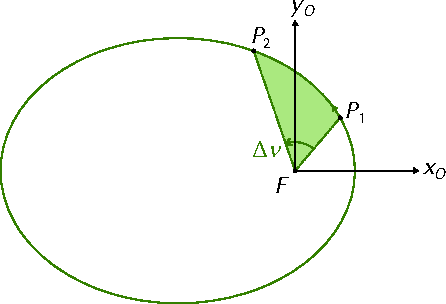
\includegraphics[scale=0.9]{fig/kepler_2.pdf}
\caption{\label{fig:kepler_2} 
Vom Radiusvektor~$(x,y)\trans$ bezüglich des Brennpunkts im Ursprung zwischen $P_1$ und $P_2$ überstrichene Fläche.
}
\end{figure}

Das \mydef{zweite Keplersche Gesetz} besagt, dass auf einer Keplerbahn über gleiche Zeiten gleiche Flächen vom Radiusvektor überstrichen werden, siehe Abb.~\ref{fig:kepler_2}.

Für den Inhalt~$A$ der in der Abbildung getönte Fläche findet man in der Tat leicht, dass
\begin{align}
	\int_A dx\wedge dy 
	&\overset{(1)}{=} \frac{1}{2}\oint (x dy - y dx)
	\overset{(2)}{=} \frac{1}{2}\oint r^2 d\Phi	
	\overset{(3)}{=} \frac{1}{2}\int_{P_1}^{P_2} r^2 d\Phi
	\nonumber\\
	&= \frac{1}{2}\int_{t_1}^{t_2} r^2\dot{\Phi}\ dt
	\overset{(4)}{=} \frac{1}{2}L\ (t_2 - t_1)
	\ .
\end{align}
Die Fläche ist somit alleine durch den erhaltenen Drehimpuls~$L$ und der bei deren Überstreichung vergangenen Zeit bestimmt.
\footnote{Schritt~(1) folgt aus dem Satz von Stokes. 
In Schritt~(2) ist auf Polarkoordinaten transformiert worden
Schritt~(3) ergibt sich daraus, dass die 1-Form $r^2d\Phi$ auf den radialen Randlinien verschwindet, und Schritt~(4) aus der Erhaltung des Drehimpulses~$L=r^2\dot{\Phi}$.}

\subsubsection{Drittes Keplersches Gesetz}

Das \mydef{dritte Keplersche Gesetz} macht eine Aussage über die Beziehung aus Bahnumlaufzeit~$T$ und großer Halbachse~$a$.
Aus den ersten beiden Keplerschen Gesetzen folgt
\begin{align}
	T &= \frac{\pi a b}{L/2}
\end{align}
und Einsetzen der Beziehungen $L=\sqrt{\mu p}=\sqrt{\mu a (1-\varepsilon^2)}$ und $b=a\sqrt{1-\varepsilon^2}$ liefert
\begin{align}
	T &= 2\pi\sqrt{\frac{a^3}{\mu}}
	\ .
\end{align}
Daraus erhalten wir das dritte Keplersche Gesetz im Kontext von Erdsatelliten: Das Verhältnis~$T^2/a^3$ ist für alle Satellitenbahnen im selben Erdpotentialfeld gleich
(und alleine durch die Erdmasse bestimmt).

Insbesondere ist die Umlaufzeit für alle Satellitenbahnen mit gleicher großer Halbachse gleich.
Dies schließt die Kreisbahn mit Radius~$a$ ein.

\subsection{Parameter ebener elliptischer Bahnen}
\label{ssec:parameter_orbital_plane}

In diesem Abschnitt stellen wir Parameter zusammen, die zur Bestimmung von Ellipsenbahnen und Punkten darauf herangezogen werden können.

\subsubsection{Parameterdefinitionen}

\begin{itemize}

\item Die \mydef{große Halbachse}~$a$ ist der längs der Apsidenlinie gemessene halbe Abstand zwischen Apoapsis und Periapsis, im Kontext erdgebundener Satelliten also zwischen Apogäum und Perigäum.

\item Die \mydef{Exzentrizität}~$\varepsilon$ gibt an, um welchen Anteil der großen Halbachse die Brennpunkte längs der Apsidenlinie vom Mittelpunkt verschoben ist.

\item Die \mydef{Perigäums\-höhe} ist durch $(1-\varepsilon)a$ gegeben.

\item Die \mydef{wahre Anomalie}~$\nu$ bestimmt die Azimutposition des Erdsatelliten relativ zum Perigäum vom Erdmittelpunkt aus, siehe Abb.~\ref{fig:ellipsen}.
Sie ist gleich der Winkeldifferenz~$\Phi - \Phi_0$ in Gl.~(\ref{eq:focal_eq_conic}).

\item Die \mydef{mittlere Anomalie}~$M$ bestimmt die Azimutposition eines fiktiven Erdsatelliten, der eine Kreisbahn mit Radius~$a$ durchläuft und das Perigäum des eigentlichen Erdsatelliten zeitgleich mit diesem durchläuft, siehe Abb.~\ref{fig:ellipsen_flaechen}.

\item Die \mydef{exzentrische Anomalie}~$E$ bezeichnet die Azimutposition, die durch Projektion Erdsatellitenposition auf die Kreisbahn des fiktiven Erdsatelliten konstruiert wird.
Diese Projektion erfolgt längs der Halbgeraden, die senkrecht zur Apsidenlinien von dieser beginnt und den Erdsatelliten als Punkt enthält, siehe Abb.~\ref{fig:ellipsen}.

\item Das \mydef{Argument des Perigäums}~$\omega$ gibt den Winkel an, um den die Apsidenlinie gegenüber der $x$-Achse verdreht ist, siehe Abb.~\ref{fig:ellipsen_arg}.
Es erscheint als~$\Phi_0$ in Gl.~(\ref{eq:focal_eq_conic}).

\end{itemize}

\begin{figure}[h]
\centering
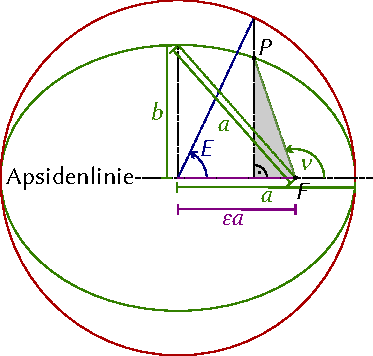
\includegraphics[scale=0.9]{fig/ellipsen.pdf}
\caption{\label{fig:ellipsen} 
Geometrische Parameter der Bahnellipsen und Position.
Die rote Kreisbahn ist die eines fiktiven Satelliten, der das Perigäum der Ellipsenbahn des eigentlichen Satelliten zeitgleich mit diesem durchläuft.
}
\end{figure}

\begin{figure}[h]
\centering
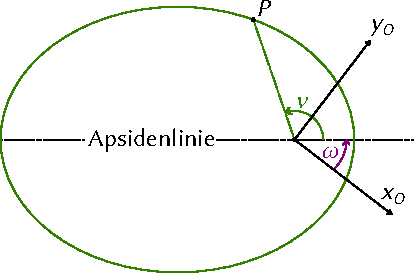
\includegraphics[scale=0.9]{fig/ellipsen_arg.pdf}
\caption{\label{fig:ellipsen_arg} 
Illustration des Arguments des Perigäums~$\omega$, das gleich der Integrationskonstante~$\Phi_0$ in Gl.~(\ref{eq:focal_eq_conic}) ist.
}
\end{figure}

\begin{figure}[h]
\centering
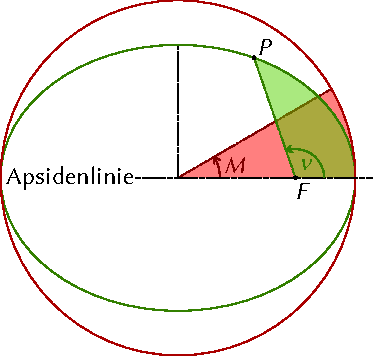
\includegraphics[scale=0.9]{fig/ellipsen_flaechen.pdf}
\caption{\label{fig:ellipsen_flaechen}
Vom Radiusvektor über die mittlere und wahre Anomalie, $M$ und $\nu$, überstrichene Flächen.
}
\end{figure}

\subsubsection{Beziehung zwischen wahrer, exzentrischer und mittlerer Anomalie}
\label{sssec:anomaly_relation}

Die vom Radiusvektor des eigentlichen Satelliten über die wahre Anomalie~$\nu$ Fläche~$A_\nu$, dargestellt als grüne Fläche in Abb.~\ref{fig:ellipsen_flaechen}, lässt sich berechnen als Differenz der gestauchten, über die exzentrische Anomalie überstrichene Fläche und der Fläche des Dreiecks aus Ellipsenmittelpunkt, -brennpunkt und Satellitenposition~$P$,
\begin{align}
	A_\nu &= \frac{a^2}{2}
	(E -\varepsilon\sin E)
	\sqrt{1-\varepsilon^2}
	\ .
\end{align}
Die vom Radiusvektor des fiktiven Satelliten über die mittlere Anomalie~$M$ überstrichene Fläche, dargestellt als rote Fläche in Abb.~\ref{fig:ellipsen_flaechen}, ist
\begin{align}
	A_M &= \frac{a^2M}{2}
	\ .
\end{align}
Nach dem dritten Keplerschen Gesetz sind die Umlaufzeiten des eigentlichen und des fiktiven Satelliten gleich.
Daher folgt aus dem zweiten Keplerschen Gesetz, dass
\begin{align}
	\frac{A_M}{\pi a^2} &= \frac{A_\nu}{\pi a b}
	\ .
\end{align}
Zusammengefasst ergibt sich die \mydef{Keplersche Gleichung}
\begin{align}
	\label{eq:mean_excentric_anomaly}
	M &= E - \varepsilon\sin E
	\ .
\end{align}
Die wahre Anomalie berechnet sich trigonometrisch anhand des in Abb.~\ref{fig:ellipsen} graugetönten Dreiecks und wir erhalten
\begin{align}
	\label{eq:true_anomaly}
	\nu &= 
	\mathrm{arctan2}(\sqrt{1-\varepsilon^2}\sin E, \cos E - \varepsilon)
	\ .
\end{align}

\subsubsection{Bestimmung der Satellitenkoordinaten}
\label{sssec:planar_coords}

Wir betrachten wiederum das kartesische Koordinatensystem~$(x, y)$ mit Ursprung im Punkt~$F$, dem Erdmittelpunkt.
Die Apsidenlinie mag gegenüber der $x$-Achse um das Argument des Perigäums~$\omega$ verdreht sein.

Den Radius~$r$ zur Satellitenposition erhalten wir zum Beispiel mit dem auf das in Abb.~\ref{fig:ellipsen} graugetönte Dreieck angewandten Satz des Pythagoras, vgl. Gl.~(\ref{eq:true_anomaly}),
\begin{align}
	\label{eq:r}
	r &= a\ (1 - \varepsilon\cos E)
	\ ,
\end{align}
während der Polarkoordinatenwinkel durch
\begin{align}
	\label{eq:phi}
	\Phi &= \nu + \omega
	\ ,
\end{align}
vgl. Abb.~\ref{fig:ellipsen_arg}, gegeben ist.
Die kartesische Koordinaten der Satellitenposition können damit mittels Gl.~(\ref{eq:polar_coord}) berechnet werden.

\subsection{Parameter im Raum geneigter elliptischer Bahnen}
\label{ssec:parameter_attitude}

Die im vorherigen Abschnitt eingeführten Parameter gestatten, einen Punkt auf einer Keplerbahn in der Bahnebene zu bestimmen.
In diesem Abschnitt kommen die Parameter hinzu, die die Lage der Bahnebene im dreidimensionalen Raum beschreiben.

\subsubsection{Parameterdefinitionen}

\begin{figure}[h]
\centering
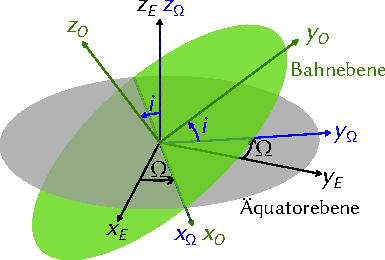
\includegraphics[scale=0.9]{fig/bahnebene.pdf}
\caption{\label{fig:orbital_attitude}
Lage der Bahnebene und seiner $x_O$- und $y_O$-Achse im räumlichen Bezugssystem mit den $x_E$-, $y_E$- und $z_E$-Achsen.
}
\end{figure}

\begin{itemize}
\item Die \mydef{Länge des aufsteigenden Knotens}~$\Omega$ bezeichnet den Lagewinkel, um den die Inklinationsachse der Bahnebene gegenüber der $x_E$-Referenzachse im räumlichen Bezugssystem verdreht ist, siehe Abb.~\ref{fig:orbital_attitude}.
Im Kontext der GNSS-Ephemeriden ist $E$ das ECEF-Koordinatensystem.
Das um $\Omega$ verdrehte System ist in Abb.~\ref{fig:orbital_attitude} mit den Indizes~$\Omega$ bezeichnet.

\item Die \mydef{Bahnneigung} oder \mydef{Inklination}~$i$ gibt den Winkel an, um den die Bahnebene gegenüber der Äquatorebene geneigt ist, siehe Abb.~\ref{fig:orbital_attitude}.

\end{itemize}
Zusammen mit dem Argument des Perigäums~$\omega$ bilden die Länge des aufsteigenden Knotens~$\Omega$ und die Bahnneigung~$i$ einen vollständigen Satz an Eulerschen Winkeln.

\subsubsection{Bestimmung der Satellitenkoordinaten}
\label{sssec:spatial_coords}

Sind die Koordinaten in der Bahnebene gegeben mit
\begin{align}
	p^O	&= 
	\begin{pmatrix}
		r\cos\Phi \\
		r\sin\Phi \\
		0
	\end{pmatrix}
	\ ,
\end{align}
vgl. Gln.~(\ref{eq:r}) und~(\ref{eq:phi}), so bleibt nur noch deren Transformation ins räumliche Koordinatensystem~$E$.
Die dazu nötigen Transformationsmatrizen lauten
\begin{align}
	C_O^\Omega &= 
	\begin{pmatrix}
		1 & 0 & 0 \\
		0 & \cos i & -\sin i \\
		0 & \sin i & \cos i
	\end{pmatrix}
	\ ,\quad
	C_\Omega^E = 
	\begin{pmatrix}
		\cos\Omega & -\sin\Omega & 0 \\
		\sin\Omega & \cos\Omega & 0 \\
		0 & 0 & 1
	\end{pmatrix}
	\ ,
\end{align}
vgl. Abb.~\ref{fig:orbital_attitude}.
Wir erhalten
\begin{align}
	p^E	&= 
	C_\Omega^E\cdot C_O^\Omega\cdot p^O
\end{align}
für die Positionskoordinaten im System~$E$.

\section{Auswertung von GNSS-Ephemeridendaten}

\subsection{Ephemeridenparameter}

Die von den betrachteten GNSS-Satelliten übertragenen Ephemeridenparameter bestehen aus sieben Parametern für eine ideale Keplerbahn und neun Korrekturparametern. 
Tabelle~\ref{tbl:ephemeris_kepler} stellt die Parameter zusammen, die mit Hilfe der gegenwärtigen, von GPS-Wochenbeginn an gemessenen Zeit die Position eines auf einer idealen Keplerbahn sich bewegenden Satelliten berechnen lässt.
In den Ephemeridendaten enthaltene Korrekturparameter sind in Tabelle~\ref{tbl:ephemeris_correction} zusammengestellt.

\begin{table}
\caption{\label{tbl:ephemeris_kepler} Ephemeridenparameter \cite{groves_2013} für eine ideale Keplerbahn.}
\centering

\begin{tabular}{|c|c|l|c|}
\hline
Symbol & Einheit & Beschreibung & Verweis \\
\hline
$t_{oe}$ & $2^4\ \mathrm{s}$ &
\parbox[t]{5cm}{Referenzzeit der Ephemeriden \\ relativ zum GPS-Wochenbeginn}
  & \\
$M_{0}$ & $2^{-31}\pi\ \mathrm{rad}$ & Mittlere Anomalie zum Zeitpunkt~$t_{oe}$ & \ref{ssec:parameter_orbital_plane} \\
$\varepsilon$ & $2^{-33}$ & Exzentrität der Ellipsenbahn & \ref{ssec:kepler_solution}, \ref{ssec:parameter_orbital_plane} \\
$\sqrt{a}$ & $2^{-19}\ \sqrt{\mathrm{m}}$ & Wurzel der großen Halbachse & \ref{ssec:kepler_solution}, \ref{ssec:parameter_orbital_plane} \\
$\Omega_0$ & $2^{-31}\pi\ \mathrm{rad}$ & 
\parbox[t]{5cm}{Länge des aufsteigenden Knotens \\ zum GPS-Wochenbeginn}  & \ref{ssec:parameter_attitude} \\
$i_0$ & $2^{-31}\pi\ \mathrm{rad}$ & Bahnneigung zum Zeitpunkt~$t_{oe}$ & \ref{ssec:parameter_attitude} \\
$\omega$ & $2^{-31}\pi\ \mathrm{rad}$ & Argument des Perigäums & \ref{ssec:parameter_orbital_plane} \\
\hline
\end{tabular}
\end{table}

\begin{table}
\caption{\label{tbl:ephemeris_correction} Ephemeridenparameter für  Korrekturen zur idealen Keplerbahn \cite{groves_2013}.
--- Anmerkung: Die Navigationsdaten der im L2C- bzx. L1C-Band von GPS versandten CNAV- und CNAV-2-Nachrichten enthalten zusätzlich die Änderungsrate~$\dot{a}$ der großen Halbachse \cite{rinex_4_02}.}
\centering

\begin{tabular}{|c|c|l|}
\hline
Symbol & Einheit & Beschreibung \\
\hline
$\Delta n$ & $2^{-43}\pi\ \mathrm{rad/s}$ & 
\parbox[t]{7cm}{Abweichung der Rate von $M$\\ vom nominalen Wert} \\
$\dot{\Omega}_d$ & $2^{-43}\pi\ \mathrm{rad/s}$ & Änderungsrate von $\Omega$ zum Zeitpunkt~$t_{oe}$ \\
$\dot{i}_d$ & $2^{-43}\pi\ \mathrm{rad/s}$ & Änderungsrate von $i$ zum Zeitpunkt~$t_{oe}$ \\
$C_{uc}$ & $2^{-29}\ \mathrm{rad}$ & 
\parbox[t]{7cm}{$\cos$-Koeffizient der harmonischen Korrektur \\ 
zur Polarkoordinate~$\Phi$, Gl.~(\ref{eq:phi})} \\
$C_{us}$ & $2^{-29}\ \mathrm{rad}$ & 
\parbox[t]{7cm}{$\sin$-Koeffizient der harmonischen Korrektur \\ 
zur Polarkoordinate~$\Phi$, Gl.~(\ref{eq:phi})} \\
$C_{rc}$ & $2^{-5}\ \mathrm{m}$ & 
\parbox[t]{7cm}{$\cos$-Koeffizient der harmonischen Korrektur \\ 
zum Bahnradius~$r$, Gl.~(\ref{eq:r})} \\
$C_{rs}$ & $2^{-5}\ \mathrm{m}$ & 
\parbox[t]{7cm}{$\sin$-Koeffizient der harmonischen Korrektur \\ 
zum Bahnradius~$r$, Gl.~(\ref{eq:r})} \\
$C_{ic}$ & $2^{-29}\ \mathrm{rad}$ & 
\parbox[t]{7cm}{$\cos$-Koeffizient der harmonischen Korrektur \\ 
zur Bahnneigung~$i$} \\
$C_{is}$ & $2^{-29}\ \mathrm{rad}$ & 
\parbox[t]{7cm}{$\sin$-Koeffizient der harmonischen Korrektur \\ 
zur Bahnneigung~$i$} \\
\hline
\end{tabular}
\end{table}


\begin{table}
\caption{\label{tbl:ephemeris_sv_clock} 
Korrekturen zur Satellitenuhr \cite{rinex_4_02}.}
\centering

\begin{tabular}{|c|c|l|c|}
\hline
Symbol & Einheit (ohne Skal.) & Beschreibung \\
\hline
$a_{f0}$ & $\mathrm{s}$ & Uhrenversatz \\
$a_{f1}$ & $\mathrm{s/s}$ & Uhrendrift \\
$a_{f2}$ & $\mathrm{s/s^2}$ & Rate der Uhrendrift \\
\hline
\end{tabular}
\end{table}

\subsection{Berechnung der Satellitenkoordinaten}

\subsection{Erdrotationskorrektur zum Empfangszeitpunkt}

\begin{thebibliography}{widest entry}
	\bibitem{groves_2013} Paul D. Groves,
	\textit{Principles of GNSS, Inertial, and Multisensor Integrated Navigation Systems}, Second Edition (2013).
	
	\bibitem{rinex_4_02} RINEX - The Receiver Independent Exchange Format, Version 4.02 (2025).

\end{thebibliography}

\end{document}